\chapter{Kiểm thử và đánh giá}
\label{chap:kiem-thu-danh-gia}
\sloppy

\section{Đánh giá thực nghiệm tầng truy hồi}
\label{sec:ch5-ke-hoach}
\label{sec:ch5-tim-kiem}

\subsection{Thiết lập thực nghiệm và kết quả các cấu hình}

Kho dữ liệu sau khi nạp 14 văn bản quy phạm pháp luật gồm 6.775 chunk, chỉ mục ngược \texttt{chunk\_terms} chứa 995.937 bản ghi âm tiết và bigram không dấu, cùng 10.570 cạnh viện dẫn nội bộ. Bộ dữ liệu đánh giá truy hồi gồm 715 câu hỏi, chia cố định thành tập \texttt{dev} (592 câu) và tập \texttt{holdout} (123 câu). Mỗi mẫu lưu câu hỏi gốc, lời gọi \texttt{search} đầu tiên do agent sinh ra khi chỉ nhìn thấy câu hỏi và mô tả công cụ, cùng danh sách đường dẫn đáp án \texttt{expected}. Một câu được tính là \textbf{tìm thấy} nếu tập kết quả chứa ít nhất một đường dẫn thuộc tập đáp án hoặc là nút con của đáp án. Độ trễ (p50, p95) được đo tuần tự trên CPU Intel Xeon W-10855M (6 nhân, 32 GB RAM), tính cả thời gian mã hóa vector truy vấn và thực thi SQL.

Bảng~\ref{tab:ch5-ablation}, Hình~\ref{fig:ch5-tim-thay} và Hình~\ref{fig:ch5-hit1} trình bày kết quả thực nghiệm ablation trên 11 cấu hình. Các cấu hình \textbf{1--4b} không có nhánh nguyên văn \texttt{verbatim\_grep} và trả về tối đa 10 điều khoản (cột ``Tìm thấy'' tương đương $\text{Hit@10}$). Các cấu hình \textbf{5--6d} trả về tối đa 10 kết quả từ nhánh hợp nhất cộng tối đa 10 kết quả bổ sung từ nhánh nguyên văn (ở thứ hạng 11--20); do đó cột ``Tìm thấy'' chỉ so sánh trực tiếp trong từng cụm (1--4b hoặc 5--6d), còn $\text{Hit@1}$ và $\text{Hit@5}$ hoàn toàn tương đương trên mọi dòng. Nếu cắt ở top 10, tỷ lệ tìm thấy của cấu hình 5 trùng với cấu hình 4 (91,0\% trên \texttt{dev}, 95,1\% trên \texttt{holdout}). Xét theo phân bố nhóm, cấu hình 5 tìm thấy 432 câu ở \texttt{both}, 107 ở \texttt{semantic\_only}, 14 ở \texttt{verbatim\_only} và trượt 39 câu trên \texttt{dev}; trên \texttt{holdout} lần lượt là 99, 18, 3 và 3 câu.

\begin{table}[htbp]
\centering
\caption{So sánh kết quả thực nghiệm của 11 cấu hình truy hồi trên tập \texttt{dev} (592 câu) và \texttt{holdout} (123 câu)}
\label{tab:ch5-ablation}
\footnotesize
\setlength{\tabcolsep}{3pt}
\begin{tabularx}{\textwidth}{@{}l >{\raggedright\arraybackslash}X r r c c r@{}}
\toprule
\multirow{2}{*}{\textbf{\#}} & \multirow{2}{*}{\textbf{Cấu hình truy hồi}} & \multicolumn{2}{c}{\textbf{Tìm thấy (\%)}} & \textbf{Dev} & \textbf{Holdout} & \textbf{p50 / p95} \\
\cmidrule(lr){3-4}
 & & \textbf{Dev} & \textbf{Holdout} & \textbf{H@1 / H@5 / MRR} & \textbf{H@1 / H@5 / MRR} & \textbf{(ms)} \\
\midrule
1 & Chỉ vector (có \texttt{query prompt}) & 83,8 & 86,2 & 50,0 / 78,4 / 0,617 & 56,9 / 83,7 / 0,673 & 364 / 515 \\
1b & Chỉ vector (không có \texttt{query prompt}) & 81,8 & 87,0 & 47,6 / 74,8 / 0,586 & 52,8 / 79,7 / 0,633 & 278 / 399 \\
2 & Chỉ từ khóa BM25 (\texttt{chunk\_terms}) & 88,7 & 92,7 & 57,8 / 80,9 / 0,681 & 61,8 / 88,6 / 0,734 & 50 / 85 \\
3 & Chỉ từ khóa \texttt{ts\_rank} (PostgreSQL) & 67,2 & 69,9 & 13,7 / 45,8 / 0,275 & 16,3 / 50,4 / 0,286 & 38 / 78 \\
4 & Kết hợp Vector + BM25 ($\text{RRF } k=20$), không có nhánh nguyên văn & 91,0 & 95,1 & 59,3 / 82,6 / 0,695 & 63,4 / 88,6 / 0,742 & 406 / 573 \\
4b & Kết hợp Vector (không prompt) + \texttt{ts\_rank} ($\text{RRF } k=60$) & 87,2 & 91,1 & 54,7 / 80,2 / 0,655 & 60,2 / 86,2 / 0,720 & 312 / 460 \\
\midrule
\textbf{5} & \textbf{Hệ thống đầy đủ (Vector có prompt + BM25, $\text{RRF } k=20$ + nguyên văn xếp theo vector)} & \textbf{93,4} & \textbf{97,6} & 58,6 / 83,8 / 0,692 & 64,2 / 88,6 / 0,751 & 501 / 690 \\
6a & Cấu hình 5, bỏ \texttt{query prompt} & 92,7 & 96,7 & 56,2 / 84,5 / 0,679 & 64,2 / 89,4 / 0,751 & 414 / 561 \\
6b & Cấu hình 5, thay bằng $\text{RRF } k=60$ & 92,7 & 97,6 & 58,4 / 83,3 / 0,690 & 64,2 / 87,8 / 0,750 & 500 / 678 \\
6c & Cấu hình 5, nhánh nguyên văn xếp theo thứ tự văn bản & 92,7 & 97,6 & 58,6 / 83,8 / 0,692 & 64,2 / 88,6 / 0,751 & 501 / 689 \\
6d & Cấu hình cơ sở (\texttt{ts\_rank}, không prompt, $\text{RRF } k=60$, nguyên văn theo thứ tự văn bản) & 90,9 & 94,3 & 56,1 / 82,4 / 0,670 & 61,0 / 85,4 / 0,720 & 404 / 562 \\
\bottomrule
\end{tabularx}
\end{table}

\begin{figure}[htbp]
\centering
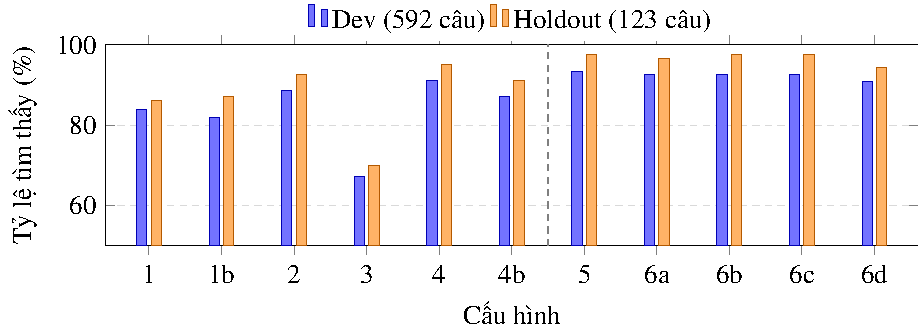
\includegraphics{graphics/fig_ch5_1.pdf}
\caption{Tỷ lệ tìm thấy đáp án theo cấu hình (dòng 1--4b: $\text{Hit@10}$; dòng 5--6d: tập kết quả đầy đủ của công cụ \texttt{search})}
\label{fig:ch5-tim-thay}
\end{figure}

\begin{figure}[htbp]
\centering
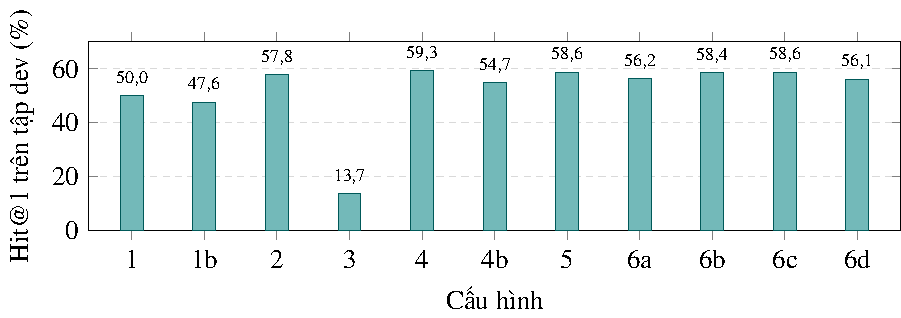
\includegraphics{graphics/fig_ch5_2.pdf}
\caption{Tỷ lệ đáp án đứng ở vị trí đầu tiên ($\text{Hit@1}$) trên tập \texttt{dev} theo từng cấu hình}
\label{fig:ch5-hit1}
\end{figure}

\subsection{Đối sánh thực nghiệm các mô hình embedding}

Bảng~\ref{tab:ch5-embedding-sweep} đối sánh mô hình \texttt{Qwen/Qwen3-Embedding-0.6B} cắt còn 512 chiều theo Matryoshka với hai mô hình cùng phân khúc 0,6 tỷ tham số giữ nguyên 1.024 chiều (\texttt{microsoft/harrier-oss-v1-0.6b} và bản tinh chỉnh chuyên biệt cho pháp luật tiếng Việt \texttt{mainguyen9/vietlegal-harrier-0.6b}) khi giữ cố định nhánh từ khóa BM25 và tập ứng viên nguyên văn. Trong bảng này, \textbf{Sem.\ H@10} và \textbf{Sem.\ MRR} đo riêng trên 10 ứng viên đứng đầu của nhánh hợp nhất RRF trước khi ghép nhánh nguyên văn.

\begin{table}[htbp]
\centering
\caption{Đối sánh 4 cấu hình mô hình embedding trong kiến trúc truy hồi kết hợp}
\label{tab:ch5-embedding-sweep}
\footnotesize
\setlength{\tabcolsep}{4pt}
\begin{tabularx}{\textwidth}{@{}>{\raggedright\arraybackslash}X c r r r r r r@{}}
\toprule
\multirow{2}{*}{\textbf{Mô hình và cấu hình}} & \multirow{2}{*}{\textbf{Chiều}} & \multicolumn{3}{c}{\textbf{Tập Dev}} & \multicolumn{3}{c}{\textbf{Tập Holdout}} \\
\cmidrule(lr){3-5}\cmidrule(l){6-8}
 & & \textbf{Phủ} & \textbf{Sem.\ H@10} & \textbf{MRR} & \textbf{Phủ} & \textbf{Sem.\ H@10} & \textbf{MRR} \\
\midrule
\textbf{\texttt{Qwen3-Embedding-0.6B} (có \texttt{Instruct})} & \textbf{512} & \textbf{93,5\%} & \textbf{90,4\%} & \textbf{0,683} & \textbf{97,7\%} & \textbf{94,6\%} & \textbf{0,696} \\
\texttt{Qwen3-Embedding-0.6B} (không prompt) & 512 & 93,0\% & 90,4\% & 0,675 & 95,4\% & 91,5\% & 0,719 \\
\texttt{harrier-oss-v1-0.6b} & 1024 & 93,8\% & 90,6\% & 0,702 & 95,4\% & 91,5\% & 0,701 \\
\texttt{vietlegal-harrier-0.6b} & 1024 & 93,3\% & 89,9\% & 0,722 & 97,7\% & 94,6\% & 0,732 \\
\bottomrule
\end{tabularx}
\end{table}

Dù chỉ sử dụng 512 chiều (giảm 50\% bộ nhớ chỉ mục HNSW và chi phí tích vô hướng), \texttt{Qwen3-Embedding-0.6B} kèm chỉ dẫn truy vấn đạt tỷ lệ tìm thấy 97,7\% và $\text{Sem.\ H@10} = 94{,}6\%$ trên tập \texttt{holdout}, ngang bằng với mô hình 1.024 chiều đã tinh chỉnh chuyên biệt trên văn bản pháp luật tiếng Việt (\texttt{vietlegal-harrier-0.6b}) và cao hơn 2,3 điểm phần trăm so với mô hình đa ngôn ngữ gốc \texttt{harrier-oss-v1-0.6b} (95,4\%). Mô hình \texttt{vietlegal-harrier-0.6b} có ưu thế nhẹ về $\text{Sem.\ MRR}$ (0,732 so với 0,696 trên \texttt{holdout}) nhờ được huấn luyện trực tiếp trên cặp câu hỏi--điều luật tiếng Việt, nhưng đòi hỏi gấp đôi dung lượng lưu trữ vector.

\subsection{Kiểm định ý nghĩa thống kê và phân tích các nhân tố}

\begin{table}[htbp]
\centering
\caption{Kiểm định McNemar chính xác ghép cặp trên toàn bộ 715 câu (\texttt{dev} và \texttt{holdout})}
\label{tab:ch5-mcnemar}
\footnotesize
\setlength{\tabcolsep}{3pt}
\begin{tabularx}{\textwidth}{@{}>{\raggedright\arraybackslash}X rrl rrl@{}}
\toprule
\multirow{2}{*}{\textbf{Cặp cấu hình so sánh}} & \multicolumn{3}{c}{\textbf{Tìm thấy}} & \multicolumn{3}{c}{\textbf{Hit@1}} \\
\cmidrule(lr){2-4}\cmidrule(l){5-7}
 & \textbf{Tốt lên} & \textbf{Kém đi} & \textbf{$p$} & \textbf{Tốt lên} & \textbf{Kém đi} & \textbf{$p$} \\
\midrule
BM25 so với \texttt{ts\_rank} (2 so với 3) & 163 & 8 & $1{,}1\cdot10^{-38}$ & 335 & 18 & $8{,}4\cdot10^{-77}$ \\
BM25 so với chỉ vector (2 so với 1) & 71 & 34 & $3{,}9\cdot10^{-4}$ & 148 & 96 & $1{,}1\cdot10^{-3}$ \\
Kết hợp Vector+BM25 so với chỉ vector (4 so với 1) & 64 & 10 & $9{,}0\cdot10^{-11}$ & 98 & 35 & $4{,}3\cdot10^{-8}$ \\
Kết hợp Vector+BM25 so với chỉ BM25 (4 so với 2) & 29 & 12 & $0{,}012$ & 71 & 60 & $0{,}38$ \\
Bổ sung nhánh nguyên văn (5 so với 4) & 17 & 0 & $1{,}5\cdot10^{-5}$ & 24 & 27 & $0{,}78$ \\
Sử dụng \texttt{query prompt} (5 so với 6a) & 7 & 2 & $0{,}18$ & 27 & 13 & $0{,}039$ \\
$\text{RRF } k=20$ so với $k=60$ (5 so với 6b) & 4 & 0 & $0{,}125$ & 3 & 2 & $1{,}0$ \\
Nhánh nguyên văn xếp theo vector (5 so với 6c) & 4 & 0 & $0{,}125$ & 0 & 0 & $1{,}0$ \\
Hệ thống đầy đủ so với cấu hình cơ sở (5 so với 6d) & 26 & 7 & $0{,}0013$ & 68 & 49 & $0{,}096$ \\
\bottomrule
\end{tabularx}
\end{table}

Từ Bảng~\ref{tab:ch5-ablation}, Bảng~\ref{tab:ch5-embedding-sweep} và Bảng~\ref{tab:ch5-mcnemar}, năm kết quả định lượng trả lời trực tiếp cho câu hỏi nghiên cứu CH1 và CH2:
\begin{enumerate}
    \item \textbf{BM25 âm tiết/bigram vượt xa \texttt{ts\_rank} ($p = 8{,}4\cdot10^{-77}$ ở $\text{Hit@1}$):} Việc \texttt{ts\_rank} thiếu trọng số IDF và chuẩn hóa độ dài khiến các từ phổ biến (\emph{``xe''}, \emph{``giao thông''}) và các đoạn quy định chung dài hàng trăm âm tiết lấn át các Điểm chế tài ngắn; thay bằng BM25 giúp $\text{Hit@1}$ nhánh từ khóa trên \texttt{dev} tăng từ 13,7\% lên 57,8\%.
    \item \textbf{Hợp nhất RRF và vai trò của bước chuẩn hóa truy vấn:} Kết hợp Vector + BM25 (dòng 4) vượt trội so với chỉ dùng vector ($p = 9{,}0\cdot10^{-11}$) và cải thiện độ phủ có ý nghĩa thống kê so với chỉ dùng BM25 ($p = 0{,}012$). Nhánh BM25 đơn lẻ cao hơn nhánh vector đơn lẻ trên bộ 715 câu vì truy vấn trong bộ đề đã được agent viết lại bằng thuật ngữ pháp lý; ngược lại, khi đưa câu hỏi thô trực tiếp vào bộ tìm kiếm một bước (\texttt{mode = "retrieve"}), $\text{Hit@1}$ giảm từ 79,5\% (trên câu hỏi sinh từ lời luật) xuống 49,3\% (trên 81 câu hỏi người dùng thật) và chỉ đạt 27,3\% trên câu không dấu, chứng minh sự cần thiết của cả bước viết lại truy vấn lẫn phép hợp nhất hai nhánh.
    \item \textbf{Nhánh nguyên văn \texttt{verbatim\_grep} cứu 17 câu khó ($p = 1{,}5\cdot10^{-5}$):} Bổ sung nhánh nguyên văn nâng tỷ lệ tìm thấy lên 93,4\% (\texttt{dev}) và 97,6\% (\texttt{holdout}) với chi phí tăng thêm $\sim 90\text{ ms}$ ở mức trung vị; xếp hạng kết quả nguyên văn theo khoảng cách cosine với vector câu hỏi (5 so với 6c) cứu thêm 4 câu khi cụm \texttt{pattern} xuất hiện ở hàng trăm đoạn (như \emph{``phục hồi điểm''} khớp toàn bộ 1.413 đoạn của Nghị định 168/2024/NĐ-CP).
    \item \textbf{Đóng góp của \texttt{query prompt} và $\text{RRF } k = 20$:} Thêm \texttt{query prompt} (5 so với 6a) tăng $\text{Hit@1}$ có ý nghĩa thống kê ($+27 / -13$, $p = 0{,}039$, thêm $\sim 85\text{ ms}$ CPU); hạ $k = 60$ xuống $k = 20$ (5 so với 6b) giữ lại 4 câu trên \texttt{dev} có đáp án đứng hạng 1--3 ở một nhánh nhưng vắng mặt ở nhánh kia.
    \item \textbf{Hiệu quả biểu diễn cây và suy diễn sửa đổi cấp Khoản/Điểm (CH1):} Rút gọn tiêu đề Chương loại bỏ chuỗi 361 ký tự lặp lại ở đầu 843 đoạn thuộc Chương II Nghị định 168/2024/NĐ-CP (chiếm 61\% độ dài trung bình chuỗi embedding). Bộ phân tích câu lệnh sửa đổi (\texttt{AmendmentIndex}) xác định 109 câu lệnh với 183 đích và gắn ghi chú cho đúng 366 chunk thực sự bị sửa, loại bỏ hoàn toàn 395/686 trường hợp gắn nhầm khi chỉ so khớp tiêu đề Điều.
\end{enumerate}

\section{Đánh giá thực nghiệm câu trả lời cuối}
\label{sec:ch5-cau-tra-loi}

\subsection{Bộ dữ liệu và tiêu chí đánh giá}

Bộ dữ liệu đánh giá câu trả lời cuối (được trích mẫu tại Phụ lục~\ref{app:cau-hoi}) gồm 81 câu hỏi độc lập với bộ truy hồi: \textbf{71 câu trong phạm vi} (36 khẩu ngữ, 15 trang trọng, 11 không dấu, 5 viết tắt, 4 suy luận nhiều bước) và \textbf{10 câu ngoài phạm vi} (án hình sự, bồi thường dân sự, bảo hiểm, luật nước ngoài). Một câu trong phạm vi được công nhận là \textbf{đúng toàn phần} khi thỏa mãn đồng thời 5 điều kiện: (1) có trích nguồn, (2) trích đúng Điều kỳ vọng, (3) nêu đủ mọi mốc tiền phạt bắt buộc, (4) nêu đủ mọi dữ kiện định lượng bắt buộc, và (5) đạt \texttt{check\_grounding}. Câu ngoài phạm vi được tính là từ chối đúng khi không trích nguồn hoặc nêu rõ kho văn bản không quy định.

\subsection{Kết quả định lượng}

\begin{table}[htbp]
\centering
\footnotesize
\setlength{\tabcolsep}{3pt}
\begin{minipage}[t]{0.58\textwidth}
\centering
\caption{Kết quả đánh giá câu trả lời cuối trên bộ 81 câu}
\label{tab:ch5-ket-qua-tra-loi}
\begin{tabularx}{\linewidth}{@{}>{\raggedright\arraybackslash}X r@{}}
\toprule
\textbf{Chỉ số đánh giá} & \textbf{Kết quả} \\
\midrule
Đúng toàn phần (71 câu trong phạm vi) & 97,2\% (69/71) \\
Trích dẫn đúng cấp Điều & 97,2\% (69/71) \\
Trích dẫn đúng cấp Khoản / Điểm & 97,2\% (69/71) \\
Đủ mức tiền phạt và dữ kiện (trên 69 câu trích đúng Điều) & 100,0\% (69/69) \\
Tỷ lệ câu trả lời có số liệu bám nguồn & 98,8\% (80/81) \\
Tỷ lệ từ chối nhầm câu hỏi trong phạm vi & 0,0\% (0/71) \\
Tỷ lệ từ chối đúng câu hỏi ngoài phạm vi & 80,0\% (8/10) \\
Thời gian phản hồi trung vị / cực đại & 36 s / 105 s \\
Chi phí suy luận tổng / trung bình mỗi câu & 12,84 / 0,159 USD \\
\bottomrule
\end{tabularx}
\end{minipage}\hfill
\begin{minipage}[t]{0.38\textwidth}
\centering
\caption{Tỷ lệ đúng toàn phần theo kiểu câu hỏi}
\label{tab:ch5-theo-kieu}
\begin{tabularx}{\linewidth}{@{}>{\raggedright\arraybackslash}X r r@{}}
\toprule
\textbf{Kiểu câu hỏi} & \textbf{Số câu} & \textbf{Tỷ lệ đúng} \\
\midrule
Khẩu ngữ & 36 & 100,0\% \\
Không dấu & 11 & 100,0\% \\
Trang trọng & 15 & 100,0\% \\
Viết tắt & 5 & 80,0\% \\
Nhiều bước & 4 & 75,0\% \\
\midrule
\textbf{Tổng cộng} & \textbf{71} & \textbf{97,2\%} \\
\bottomrule
\end{tabularx}
\end{minipage}
\end{table}

Cả ba nhóm câu hỏi phổ biến nhất (khẩu ngữ, không dấu, trang trọng) đều đạt 100,0\% nhờ bước agent tự biên dịch câu hỏi đời thường sang thuật ngữ pháp lý trước khi gọi \texttt{search}.

\subsection{So sánh truy hồi một bước với điều phối agent đa bước}

\begin{table}[htbp]
\centering
\caption{Đối sánh ghép cặp giữa lời gọi \texttt{search} đầu tiên và điều phối agent đa bước trên 40 câu \texttt{holdout}}
\label{tab:ch5-so-sanh}
\footnotesize
\begin{tabularx}{\textwidth}{@{}>{\raggedright\arraybackslash}X r r@{}}
\toprule
\textbf{Tiêu chí đo lường} & \textbf{Lời gọi \texttt{search} đầu tiên} & \textbf{Agent tra cứu đa bước} \\
\midrule
Tỷ lệ điều khoản đáp án được tìm thấy / được chọn trích dẫn & 95,0\% (38/40) & 92,5\% (37/40) \\
Số câu agent đa bước cứu được / làm lệch đi so với lần gọi đầu & -- & 1 câu / 2 câu \\
Độ trễ thực thi trung vị mỗi câu & $< 1\text{ giây}$ (sau khi có truy vấn) & $\approx 36\text{ giây}$ (trung bình 3,8 lượt) \\
Chi phí suy luận trung bình mỗi câu & 1 lượt sinh truy vấn & $\approx 0{,}16\text{ USD}$ \\
\bottomrule
\end{tabularx}
\end{table}

Bảng~\ref{tab:ch5-so-sanh} cho thấy ngay ở lời gọi \texttt{search} đầu tiên do agent viết, bộ truy hồi kết hợp đã tìm thấy đáp án cho 95,0\% số câu; các lượt gọi công cụ tiếp theo không làm tăng tỷ lệ định vị đường dẫn (92,5\%), nhưng đóng vai trò quyết định ở tầng tổng hợp câu trả lời: dùng \texttt{hierarchical\_navigate} đọc toàn văn Điều/Khoản để lấy khung phạt và hình thức phạt bổ sung, đi theo viện dẫn qua \texttt{graph\_traverse}, đọc điều khoản sửa đổi từ \texttt{amended\_by} và tự hiệu chỉnh khi \texttt{check\_grounding} báo lỗi.

\section{Phân tích lỗi và hạn chế}
\label{sec:ch5-phan-tich-loi}
\label{sec:ch5-danh-gia-chung}

\subsection{Phân tích các trường hợp lệch trên bộ câu trả lời cuối}

\begin{table}[htbp]
\centering
\caption{Phân tích chi tiết 4 câu trả lời lệch so với đáp án kỳ vọng (2 câu trong phạm vi, 2 câu ngoài phạm vi)}
\label{tab:ch5-loi-tra-loi}
\footnotesize
\setlength{\tabcolsep}{4pt}
\begin{tabularx}{\textwidth}{@{}l >{\raggedright\arraybackslash}p{2.4cm} >{\raggedright\arraybackslash}X >{\raggedright\arraybackslash}p{3.6cm}@{}}
\toprule
\textbf{Mã} & \textbf{Phán quyết} & \textbf{Nội dung câu trả lời thực tế của hệ thống} & \textbf{Nguyên nhân gốc} \\
\midrule
\texttt{u045} & Trích khác Điều kỳ vọng & Hỏi \emph{``quên mang bằng lái nhưng có trên VNeID thì có bị phạt ko''}: agent trích Điều 48 Nghị định 168/2024/NĐ-CP (thủ tục kiểm tra giấy tờ tích hợp định danh điện tử) thay vì Khoản 3 Điều 56 Luật TTATGTĐB & Đáp án kỳ vọng chỉ ghi Điều 56 Luật TTATGTĐB, chưa đưa Điều 48 Nghị định 168 vào tập chấp nhận \\
\texttt{u070} & Trích khác Điều và có 1 số Điều vượt nguồn & Hỏi \emph{``Nghị định 100/2019 còn hiệu lực không''}: agent trích Điều 52 Nghị định 168/2024/NĐ-CP và liệt kê đúng các điều khoản bị bãi bỏ, nhưng nhắc tới ``Điều 25'' thuộc Điểm i Khoản 8 Điều 52 mà chưa đưa điểm lá này vào \texttt{sources} & Đáp án kỳ vọng chỉ ghi Điều 53, 54; đồng thời agent trích thiếu 1 điểm lá trong cùng Điều 52 \\
\texttt{o002}, \texttt{o004} & Không từ chối (ngoài phạm vi) & Hỏi mức bồi thường tai nạn chết người / va quẹt trầy sơn xe: agent trả lời rõ văn bản trong kho không quy định mức bồi thường dân sự nhưng vẫn đính kèm điều khoản nguồn về nghĩa vụ khi xảy ra tai nạn & Câu trả lời trung thực nhưng tiêu chí chấm yêu cầu câu ngoài phạm vi không được đính kèm nguồn tham khảo \\
\bottomrule
\end{tabularx}
\end{table}

Trên toàn bộ 71 câu trong phạm vi, \textbf{không có bất kỳ câu trả lời nào trích dẫn sai quy định, nêu sai khung tiền phạt hoặc tự bịa số liệu}.

\subsection{Phân tích các trường hợp truy hồi trượt và hạn chế của đề tài}

\begin{table}[htbp]
\centering
\caption{Phân loại nguyên nhân gốc của các câu truy hồi trượt trên tập \texttt{dev}}
\label{tab:ch5-loi-tim-kiem}
\footnotesize
\setlength{\tabcolsep}{4pt}
\begin{tabularx}{\textwidth}{@{}>{\raggedright\arraybackslash}X r >{\raggedright\arraybackslash}p{3.6cm} >{\raggedright\arraybackslash}p{4.4cm}@{}}
\toprule
\textbf{Nhóm nguyên nhân gốc} & \textbf{Số câu} & \textbf{Trường hợp điển hình} & \textbf{Cơ chế xử lý} \\
\midrule
Nhánh nguyên văn cắt 10 kết quả đầu theo thứ tự văn bản & $\sim 17$ & Cụm \emph{``phục hồi điểm''} khớp 1.413 đoạn do nằm trong tiêu đề Nghị định 168/2024/NĐ-CP & Sắp xếp kết quả \texttt{verbatim\_grep} theo khoảng cách cosine với vector câu hỏi \\
Phép hợp nhất RRF với $k=60$ làm rơi ứng viên hạng 1--3 của một nhánh khỏi top 10 & $\sim 15$ & Mẫu \texttt{e308}: đứng hạng 2 ở nhánh vector nhưng rơi xuống hạng 12 sau khi gộp với nhánh từ khóa & Giảm hằng số làm mượt xuống $\text{RRF } k=20$ \\
Hàm \texttt{ts\_rank} thiếu trọng số IDF và chuẩn hóa độ dài & $\sim 6$ & Mẫu \texttt{e075}: đứng hạng 1 theo vector nhưng hạng 226 theo \texttt{ts\_rank} do các từ phổ biến lấn át & Thay bằng chỉ mục ngược \texttt{chunk\_terms} và hàm điểm BM25 \\
Biểu diễn vector của mô hình 0.6B chưa phân biệt được các điều khoản có câu dẫn dài tương tự nhau & $\sim 9$ & Khoản 10 Điều 32 Nghị định 168/2024/NĐ-CP rơi xuống hạng 742--880 trên nhánh vector & Tầng agent khắc phục qua \texttt{hierarchical\_navigate}; tầng truy hồi cần mô hình lớn hơn hoặc reranker \\
Truy vấn đầu vào chọn từ khóa hoặc phạm vi \texttt{doc\_codes} chưa sát & 3 & Từ \emph{``đường nhánh''} trong câu hỏi bị viết lại thành \emph{``đường cao tốc''} & Thuộc bước sinh truy vấn của agent, không thuộc hàm xếp hạng \\
Nhãn đáp án kỳ vọng (\texttt{expected}) ghi thiếu điều khoản tương đương & 3 & Các mẫu \texttt{e165}, \texttt{e537}, \texttt{e186} & Bổ sung điều khoản tương đương khi thẩm định chuyên môn \\
\bottomrule
\end{tabularx}
\end{table}

Hệ thống hiện còn bốn hạn chế chính: (1) bộ đáp án của tập truy hồi và 81 câu trả lời chưa qua bước thẩm định độc lập của chuyên gia pháp lý (đã ghi nhận 3 mẫu truy hồi và 2 câu trả lời \texttt{u045}, \texttt{u070} có tập điều khoản kỳ vọng hẹp hơn thực tế); (2) các biểu mẫu hành chính (\texttt{Mẫu số...}) mới được nhận diện để loại trừ chứ chưa bóc tách trường thông tin bên trong; (3) chế độ agent còn phụ thuộc vào mô hình thương mại với độ trễ trung vị 36 giây; và (4) bộ suy diễn sửa đổi chưa giải các câu lệnh sửa đổi cấp Chương/Mục hoặc chuỗi văn bản sửa đổi bắc cầu, đồng thời ở chế độ một bước (\texttt{retrieve}), việc lọc câu hỏi ngoài miền chỉ dựa được vào dấu hiệu khớp cụm âm tiết do điểm tương đồng cosine của \texttt{Qwen3-Embedding-0.6B} luôn cao trên tiền tố văn bản chung.

\fussy
